Une fois la simulation lancée. Le tick 1 crée la position de départ du peuplement. Le tick 2 crée les agents. Il est possible, à partir du tick 3, de sélectionner un agent (avec un clic gauche) et de l'observer (au moyen d'un clic droit suivi de la sélection du choix \textit{Observe one agent}). Cette fenêtre d'observation se met à jour automatiquement à chaque tick de la simulation. Elle permet ainsi d'observer facilement l'évolution d'un ou plusieurs agents au cours de la simulation.

\subsection{La fenêtre d'observation d'un agent}

Le premier onglet, l'onglet \textit{Mind}, qui s'ouvre automatiquement, représente les cognitons et les plans présents dans l'esprit de l'agent. Il permet d'observer rapidement la répartition des cognitons et des plans dans l'esprit de l'agent (cf. Figure \ref{observe}).

\begin{figure}[!ht]
\begin{center}
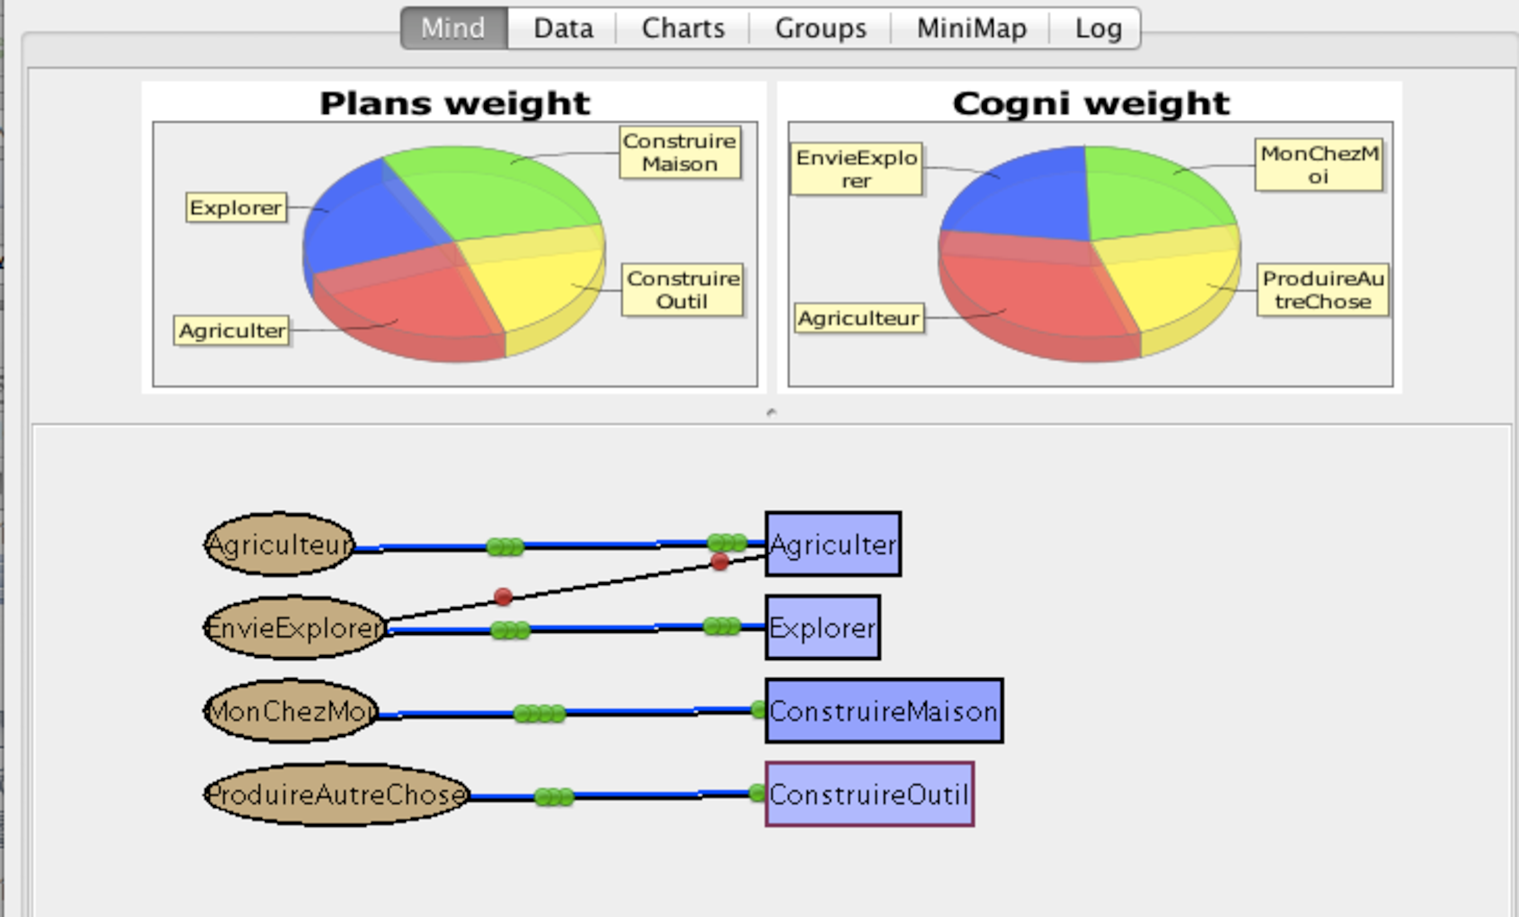
\includegraphics[scale=0.5]{DocumentationSimulation/observe.pdf}
\caption[observe]{Fenêtre d'observation de la constitution de l'esprit de l'agent \\}
\label{observe}
\end{center}
\end{figure} 

Cela permet ainsi, au moyen du graphique \textit{Cogni weight}, de voir que, au tick auquel a été prise cette impression d'écran, l'agent observé possédait les quatre cognitons EnvieExplorer, Agriculteur, MonChezMoi et ProduireAutreChose avec un poids un peu plus important pour le cogniton Agriculteur. De même on peut aussi voir que cet agent est susceptible, à ce tick, d'effectuer les plans Explorer,Construire Outil, Construire Maison et Agriculter avec un peu plus de chances pour le plan Construire Maison et Agriculter. 


L'onglet \textit{Data }présente une vision globale des données concernant l'agent, à savoir, le poids de ses cognitons, le poids des plans qu'il est susceptible d'effectuer, la valeur de chacun de ses attributs, son inventaire, le plan qu'il effectue au cours de ce tick, ainsi que le type de patch sur lequel il se trouve (cf. Figure \ref{observe2}) ou même les groupes auxquels il appartient.

\begin{figure}[!ht]
\begin{center}
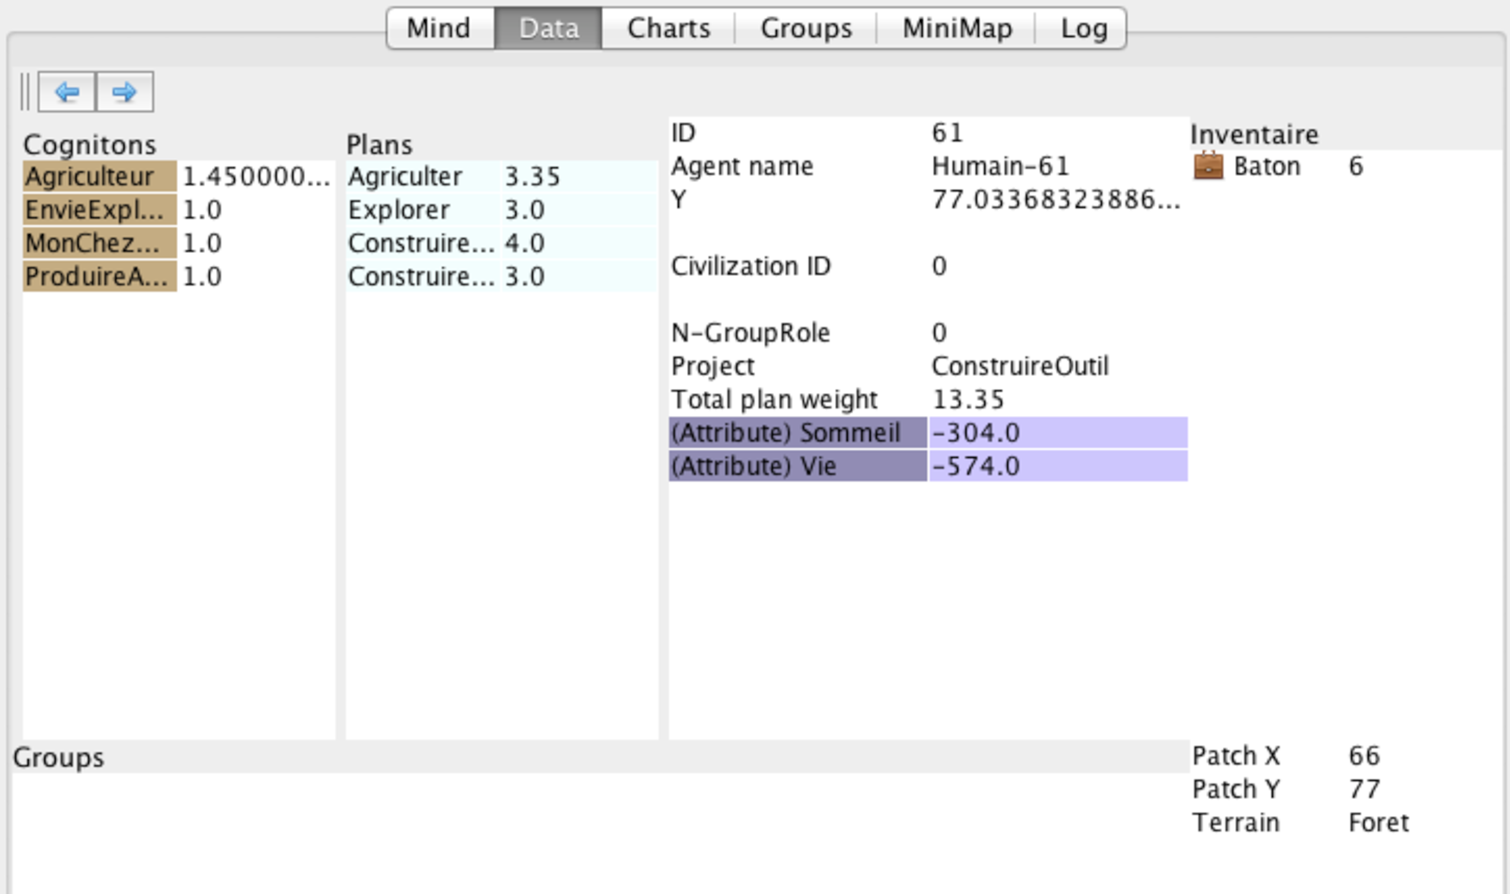
\includegraphics[scale=0.5]{DocumentationSimulation/observe2.pdf}
\caption[observe]{Fenêtre d'observation de l'agent \\}
\label{observe2}
\end{center}
\end{figure} 

Dans le cas de cette simulation et à ce tick précis, on peut voir que l'agent observé possède le cogniton Agriculteur, lequel a un poids de 1.45, les autres cognitons présents dans l'esprit de l'agent ont un poids de 1.0 ce qui confirme l'information donnée par le premier onglet, il en est de même concernant les plans. On peut aussi constater que l'agent possède 6 objets Bâton dans son inventaire et que son plan actuel est Construire\_Outil. Il est donc prévisible qu'au prochain tick, l'agent crée un outil à partir de ces bâtons. De plus on observe que l'agent possède ces deux attributs Vie et Sommeil largement en négatif, ce qui est normal, car rien n'a été  prévu, dans cette simulation, lors de la création de la cognition de l'agent, pour pousser ce dernier à consommer de la nourriture ou à aller se reposer si ses attributs atteignent un seuil critique. Il aurait été possible de le faire en définissant un \textit{trigger } portant sur l'attribut voulu et déclenchant l'apparition d'un cogniton influençant très positivement un plan consistant à augmenter la valeur de cet attribut. Enfin cet onglet nous permet de constater que l'agent n'appartient à aucun groupe et qu'il se situe sur un patch de type Forêt.

L'onglet \textit{Charts} contient deux graphiques représentant, pour le premier, la répartition des attributs de l'agent, et le second, un aperçu rapide de la valeur de chaque plan de l'agent. Passer la souris sur chaque composante des graphiques permet d'obtenir plus d'informations (cf. Figure \ref{observe3}).

\begin{figure}[!ht]
\begin{center}
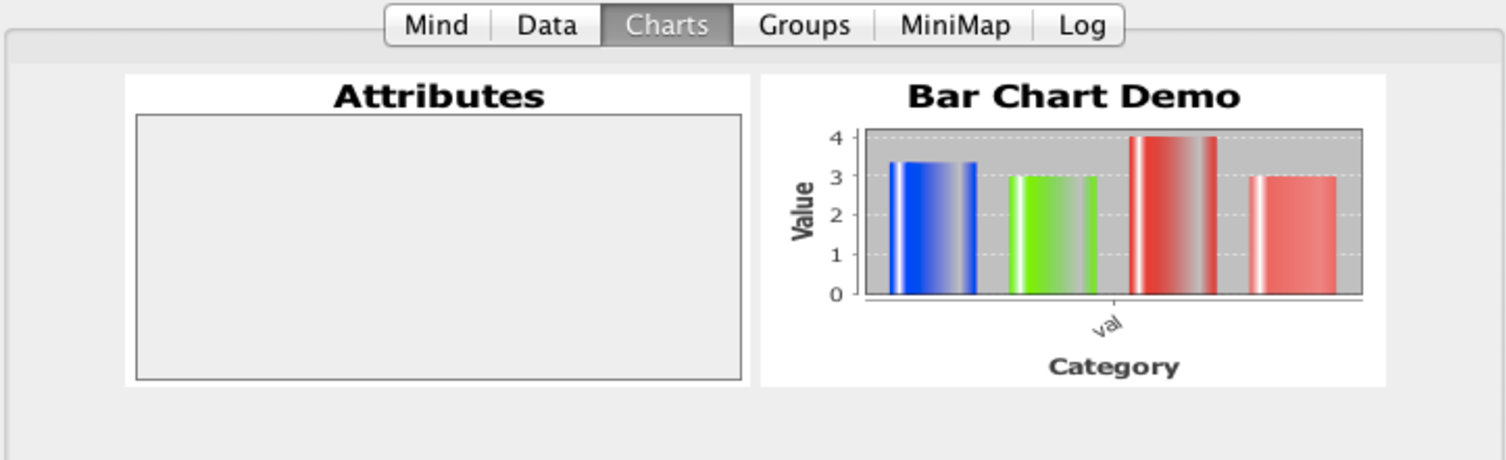
\includegraphics[scale=0.5]{DocumentationSimulation/observe3.pdf}
\caption[observe]{Fenêtre d'observation des attributs et plans de l'agent \\}
\label{observe3}
\end{center}
\end{figure} 

Cet onglet permet ainsi de confirmer que les valeurs des attributs de l'agent sont négatives car elles n'apparaissent pas dans le graphique et nous montre le poids de chaque plan susceptible d'être effectué par l'agent sous forme d'un diagramme. Pour savoir quel plan est représenté par quelle couleur il suffit de passer la souris au-dessus de celui-ci.



L'onglet \textit{Groups} permet d'avoir une représentation des groupes auxquels appartient l'agent observé, ainsi que son rôle dans ces groupes. L'agent n'appartenant à aucun groupe cet onglet ne nous apprendra rien dans cette simulation, dans d'autres simulations nous pourrions observer les rôles de l'agent observé dans les différents groupes auxquels il appartiendrait.



L'onglet \textit{Minimap} permet d'avoir un zoom sur la position de l'agent sur la carte.



Enfin, l'onglet \textit{Log }permet d'avoir un récapitulatif des plans et des actions effectués par l'agent à chaque tick (cf. Figure \ref{observe4}).

\begin{figure}[!ht]
\begin{center}
\includegraphics[scale=0.5]{DocumentationSimulation/observe4.pdf}
\caption[observe]{Fenêtre récapitulative des actions de l'agent \\}
\label{observe4}
\end{center}
\end{figure} 

Nous pouvons ainsi voir que les derniers agissements de l'agent consistaient à aller se reposer à sa maison puis à aller chercher de quoi fabriquer des outils.


\subsection{La fenêtre d'observation générale}

Il est aussi possible d'observer le comportement général des agents au moyen des onglets \textit{Agents}, \textit{Options}, \textit{Performances}, \textit{Tableau de bord} et \textit{Charts} présentés précedemment.

L'onglet \textit{Agents} correspond à l'onglet \textit{Data} présenté précédemment à ceci prés qu'il est muni de deux flèches avant et arrière permettant de facilement passer de l'observation d'un agent à un autre.

L'onglet \textit{Options} permet de définir les préférences d'affichage de la fenêtre \textit{WorldViewer}. Il est muni de plusieurs options :
\begin{itemize}
\item \textit{Affichage des plans} : permet de n'afficher que les agents effectuant un certain plan à sélectionner dans la liste déroulante. Les agents n'effectuant pas ce plan seront minimisés et ne seront visibles qu'en cas de zoom.
\item \textit{PheroMap} : permet de colorer les patches non plus en fonction de leur type de terrain mais en fonction de la valeur de la ressource sélectionnée pour chaque patch. Plus la ressource est présente sur le patch, plus ce dernier sera coloré en bleu.
\item \textit{ShowSpecificGroupAndRole} : permet de colorer les agents en fonction de leur appartenance à un groupe.
\end{itemize}

L'onglet \textit{Performances} quand à lui affiche les ressources matérielles utilisées par la simulation.

L'onglet \textit{Tableau de bord} permet, en cliquant sur l'icône \textit{Mettre à jour les données} représentée par une double disquette, de visualiser pour chaque cogniton, le pourcentage d'agents présents dans la simulation le possédant. 
% à voir

Enfin l'onglet \textit{Charts} permet de voir l'évolution de la moyenne des poids de chaque plan dans l'esprit des agents composants la simulation, de même pour les attributs.

\subsection{La fenêtre d'observation avancée}

Dans l'onglet Charts se trouves aussi un bouton qui donnes accès à l'observation avancée de la simulation


\begin{figure}[!ht]
\begin{center}
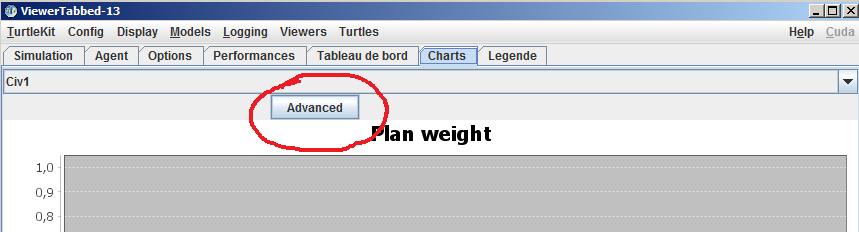
\includegraphics[scale=0.5]{DocumentationSimulation/images/accesAdvStats.png}
\caption[observe]{Accès à la fenêtre d'observation avancée\\}
\label{observe5}
\end{center}
\end{figure} 



\begin{figure}[!ht]
\begin{center}
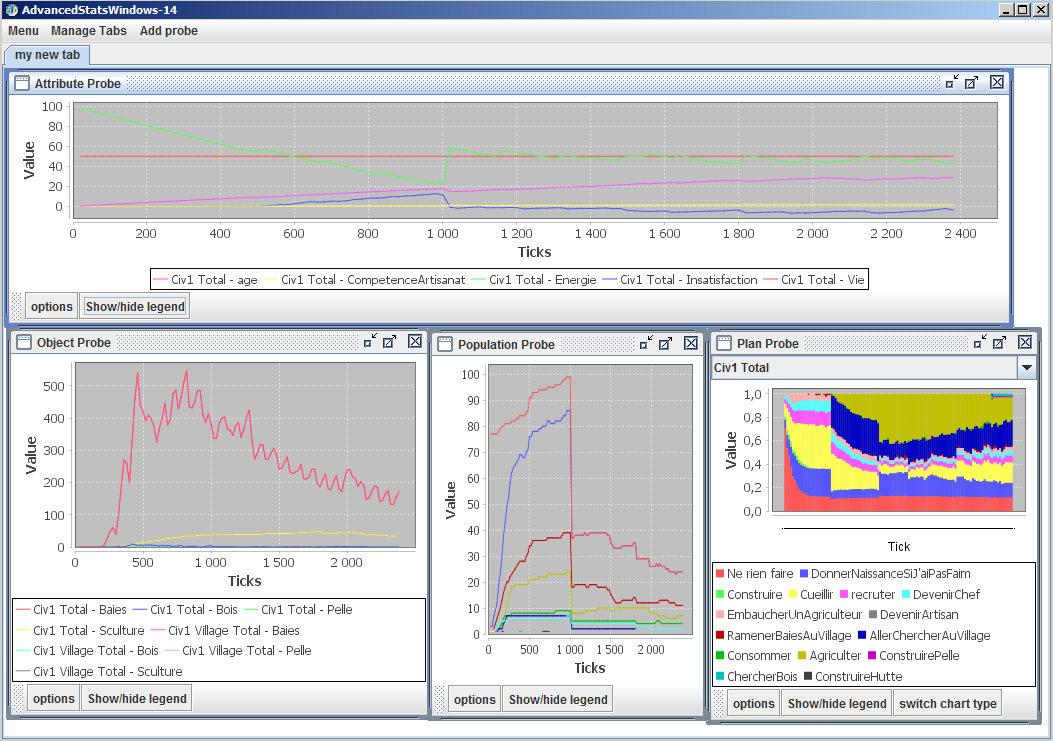
\includegraphics[scale=0.5]{DocumentationSimulation/images/ADVS_Exemple.png}
\caption[observe]{Exemple de visualisation\\}
\label{observe6}
\end{center}
\end{figure} 
\newpage
\subsubsection{Exemple de mise en place}

Tout d'abord , il est recommandé de créer un onglet dédié à ce que nous souhaitons observer.

\begin{figure}[!ht]
\begin{center}
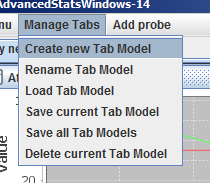
\includegraphics[scale=0.8]{DocumentationSimulation/images/ADVS_tabs.png}
\caption[observe]{Menu de gestion des onglets\\}
\label{observe7}
\end{center}
\end{figure} 

Le menu de gestion des onglets permet de créer un nouvel onglet , de sauvegarder le modèle d'onglet courant , ou de sauvegarder tous les modèles d'onglets ouverts

La création d'un onglet demandes d'entrer un nom pour l'onglet

\begin{figure}[!ht]
\begin{center}
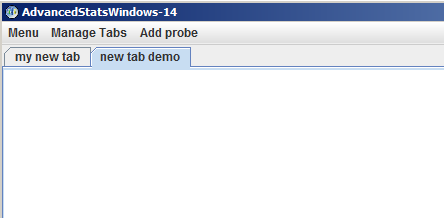
\includegraphics[scale=0.8]{DocumentationSimulation/images/ADVS_newTab.png}
\caption[observe]{Un nouvel onglet vierge\\}
\label{observe8}
\end{center}
\end{figure} 

Le menu des sondes (add probe) permet choisir différents types de sondes

\begin{figure}[!ht]
\begin{center}
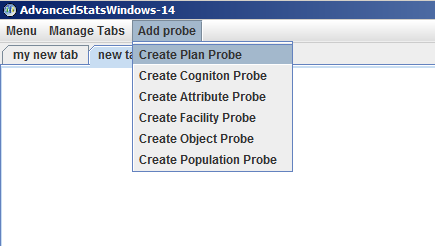
\includegraphics[scale=0.8]{DocumentationSimulation/images/ADVS_ProbeMenu.png}
\caption[observe]{Le menu des sondes\\}
\label{observe9}
\end{center}
\end{figure} 

\begin{itemize}
\item  Create plan probe : permet d'observer le poids des plans dans l'esprit des agents
\item  Create cogniton probe : permet d'observer le poids des cognitons dans l'esprit des agents
\item  Create attribute probe : permet d'observer la valeur des attributs dans des agents
\item  Create object probe : permet d'observer la quantité d'objets dans l'inventaire des agents
\item  Create population probe : permet compter le nombre d'agents
\end{itemize}

Nous allons créer une sonde sur les population.
Dans les options de toutes les sondes se trouves un onglet filtre social qui permet d'effectuer les observations de la sonde sur différents groupes sociaux du modèle.
\newpage
\begin{figure}[!ht]
\begin{center}
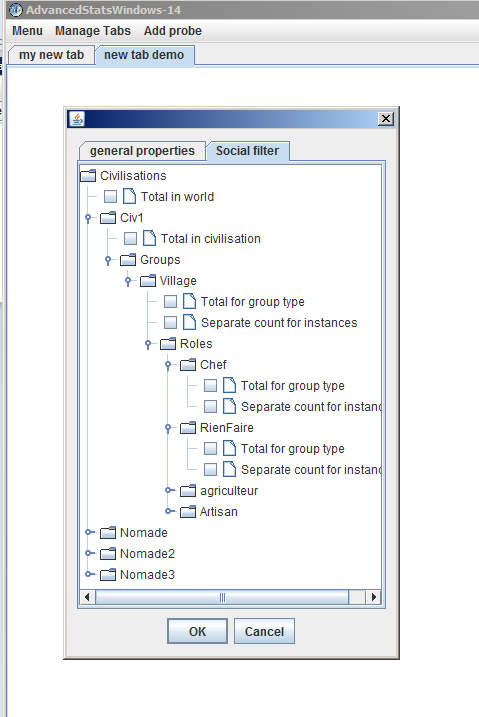
\includegraphics[scale=0.7]{DocumentationSimulation/images/ADVS_SocFilter.png}
\caption[observe]{Le filtre social\\}
\label{observe10}
\end{center}
\end{figure} 

A la racine de l'arbre se trouves l'option Total In World qui créé un compte pour tout les agents du modèle, ainsi qu'un noeud pour chaque civilisation présente dans le modèle.
\\
Dans chaque noeuds civilisation se trouve l'option Total in civilisation qui crée un compte pour tout les membres de la civilisation concernée. Dans le noeud groupe sont listés tous les types de groupes.
\\ Pour chaque groupe l'option total for group type créé un compte qui regroupes tous les agent qui appartiennent à un groupe du type sélectionné. L'option separate count for instance permet de créer un compte différent pour chaque groupe concret qui sera identifié par son type et son nom unique. Dans le noeud Roles sont listés tous les types de role du type de groupe sélectionné.
\\ Enfin ,  pour chaque role l'option Total for group type permet de créer un compte pour tout les agents ayant le role sélectionné dans tous les groupes de type sélectionné. l'option Separate count for instances permet de faire un compte séparé pour chaque instance de groupes.

\newpage
\begin{figure}[!ht]
\begin{center}
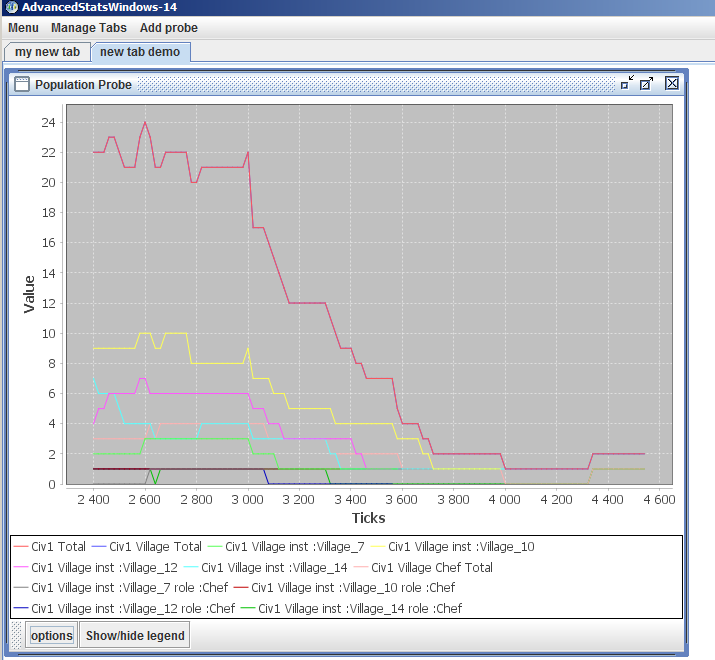
\includegraphics[scale=0.6]{DocumentationSimulation/images/ADVS_PopProbe.png}
\caption[observe]{Une sonde sur les populations\\}
\label{observe11}
\end{center}
\end{figure} 



Sur la figure précédente on peut voir grâce à la légende que total in civilisation a été sélectionné pour "Civ"1 (Civ1 Total), l'option total for groupe type pour le type Village (Civ1 Village Total),l'option separate count for instance pour le type Village (Civ1 Village inst: Village\_ XX), l'option total for groupe type pour le role Chef (Civ1 Village Chef Total) et enfin l'option separate count for instance pour le role Chef(Civ1 Village inst: Village\_ XX role: Chef) 



